\section{Description}
\subsection{Qu'est ce que c'est ?}
\textsl{Lyon Ray Tracer}, en hommage à ma ville natale : Lyon, est un moteur
de rendu utilisant la technique du \textsl{ray tracing} pour produire des
images photoréalistes. Pour ceux qui ne connaissent pas encore le \textsl{ray
tracing}, je vous invite à consulter notre ami \textsl{Wikipedia}
(\url{http://fr.wikipedia.org/wiki/Lancer_de_rayon}).

Par conséquent, mon moteur prend en entrée des informations comme ``il existe
une sphère de centre (0,0,0) et de rayon 10 qui possède un coefficient de
réflexion de 0.5'', et produit le genre d'image de la figure
\ref{fig:spheres}.

\begin{figure}
\begin{center}
  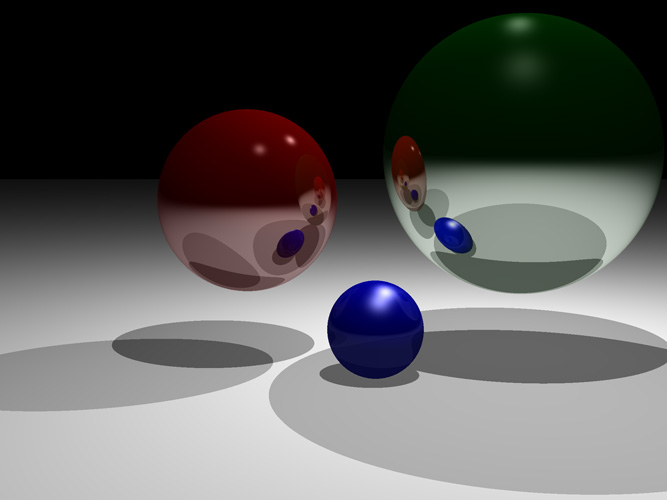
\includegraphics[width=.8\textwidth]{img/spheres}
  \caption{Un exemple de rendu en \textsl{ray tracing}\label{fig:spheres}}
\end{center}
\end{figure}

\subsection{Pourquoi ?}
Bien évidemment parce que j'aime ça ! Mon école ma proposé de réaliser le
projet de mon choix et c'est ce que j'ai choisi. De plus, je trouve que le
concept est formidable : Créer à partir de quelques informations textuelles
des images ultra réalistes et respectant les principes physiques de propagation
de la lumière.

\subsection{Comment ?}
En C++ et en utilisant le plus d'outils libres et standards. Pour vous donner
une idée de mon toolkit, je vous conseil d'aller jeter un coup d'œil du côté
des dépendances.

\subsection{C'est cool, je peux participer ??}
Oh oui !\\

Un moteur de \textsl{ray tracing} c'est comme des Légo, on peu toujours
ajouter quelques choses (surtout en ce moment, puisque le moteur n'est pas
encore très évolué). C'est donc pour toi l'occasion de participer à quelques
choses au tout début de son évolution.\\

Tu peux par exemple :
\begin{itemize}
  \item Me suivre sur GitHub ou me laisser un petit mail pour m'encourager !
  \item Essayer de compiler le programme et m'avertir des différents problèmes
    que tu as pu rencontrer (si possible avec la solution ;) )
  \item M'envoyer des \textsl{pull requests} (même si c'est pour un coquille
    ou ajouter un peu de documentation).
  \item M'aider à créer une vraie page web au lieux de ce PDF :p
\end{itemize}

\subsection{Fonctionnalités}
\paragraph{Lumières}
\begin{itemize}
  \item Lumière directionnelle.
  \item Lumière ponctuelle.
\end{itemize}

\paragraph{Caméra}
\begin{itemize}
  \item Caméra classique avec prise en compte de la perspective.
\end{itemize}

\paragraph{Géométrie}
\begin{itemize}
  \item Sphère.
  \item Plan infini.
  \item Boite.
  \item Triangle.
  \item Mesh (avec Octree).
\end{itemize}

\paragraph{Matériaux}
\begin{itemize}
  \item Couleur diffuse, spéculaire, ambiante.
  \item Indice de réfraction.
  \item Indice de réflexion.
\end{itemize}

\paragraph{Importeurs de scènes}
\begin{itemize}
  \item XML.
\end{itemize}

\paragraph{Importeurs de modèles}
\begin{itemize}
  \item 3DS.
\end{itemize}

\paragraph{Exporteurs}
\begin{itemize}
  \item PNG.
  \item JPG.
\end{itemize}
